\documentclass[10pt,a4paper]{article}
\usepackage{graphicx}
\usepackage[default]{sourcesanspro}
\usepackage{amsmath}
\usepackage{amssymb}
\usepackage[margin=0.3in]{geometry}
\usepackage[explicit]{titlesec}
\usepackage{multicol}
\usepackage{pdflscape}
\usepackage{ncolor}
\usepackage{wrapfig}
\usepackage{enumitem}
\setlist{nosep}

\linespread{1}

\newcommand{\vrulefill}[1]{\leavevmode\leaders\hrule height#1\hfill\kern0pt}
\newcommand{\firstletter}[1]{\primary#1\black}
\titleformat{\section}{\bfseries\primary}{\thesection.}{0.75em}{#1\quad\vrulefill{0.12em}}
\titlespacing*{\section}{0em}{0em}{0em}
\titleformat{\subsection}{\bfseries\primary}{\thesection.\thesubsection.}{0.75em}{#1}
\titlespacing*{\subsection}{0em}{0em}{0em}
\def\myfirstletter#1{\primary#1\black}
\DeclareRobustCommand{\FirstPrimaryLetter}[1]{\myfirstletter #1}
\titleformat{\subsubsection}[hang]{\bfseries}{\thesection.\thesubsection.\thesubsubsection.}{0.75em}{\quad\FirstPrimaryLetter#1}
\titlespacing*{\subsubsection}{0em}{0em}{0em}

\begin{document}
\begin{landscape}
\begin{multicols}{3}

\section{Process Models}
\subsection{Agile}
\begin{itemize}
    \item Embrace change -- requirements never fixed
    \item Deliver early and deliver often
\end{itemize}
\subsection{Lean}
\begin{itemize}
    \item Think big, act small, fail fast
\end{itemize}

\section{Ethics}
\subsection{Australian Computer Society (ACS)}
\begin{itemize}
    \item Primary of Public Interest
    \item Enhancement of Quality of Life
    \item Honesty
    \item Competence
    \item Professional Development
    \item Professionalism
\end{itemize}

\section{Requirements}
\subsection{Functional Requirements}
\begin{itemize}
    \item Requirements (or capabilities) for functions (specific behaviour) that must be performed by the system
    \item Primary focus of most requirements activities
\end{itemize}
\subsection{Non-Functional Requirements}
Constraints on performance or quality
\begin{itemize}
    \item Product Properties -- Requirements on the behaviour of the product (min 8 transactions per second)
    \item Process Properties -- Requirements on the practices used to develop / produce the system (Follow a standard)
\end{itemize}

\section{Elicitation}
\subsection{Interviews}
Effective for understanding problem and eliciting general requirements
\subsection{Workshops}
Multiple stakeholders; resolve conflicting requirements, quickly gather broad system usage
\subsection{Focus Groups}
Broad stakeholder representation. Gather broad-based ideas
\subsection{Observations}
Time consuming. Users often cannot describe everything they do.
\subsection{Questionnaires}
Inexpensive and easily administered to remote sites. Good questionnaires difficult to write
\subsection{System Interface Analysis}
Look at other system's functionality
\subsection{User Interface Analysis}
Study existing systems. What should be replicated and avoided
\subsection{Document Analysis}
Existing system documentation. Industry standards or legislation

\section{Use Cases}
\subsection{$<<$include$>>$ relationship}
Factor out common behaviour in use cases (scenario always uses included steps)
\subsection{$<<$extend$>>$ relationship}
Factors out optional behaviour in use cases (when there are optional or uncommon steps)

\section{Prioritisation}
\subsection{MoSCoW}
Must have, Should have, Could have, Won't have

\section{Review}
\subsection{Types of Reviews}
\subsubsection{Technical Review}
Review for conformance to standards or achievement of project milestones
\subsubsection{Software (Fagan) Inspection}
Peer review with formal process. Focus on defect detection and description
\subsubsection{Structured Walkthrough}
Less formal than inspection. No formal data collection
\subsubsection{Audit}
External review of work product. Usually late in the process
\subsection{Inspection Participants}
\subsubsection{Moderator}
Responsible for leading inspection process
\subsubsection{Recorder}
Keeps records of all significant inspection results
\subsubsection{Producer}
Responsible for work under review
\subsubsection{Reader}
Presents work instead of producer in formal inspection
\subsubsection{Reviewers}
Directly concerned with, and aware of work under review
\subsection{Inspection Process}
Request $\rightarrow$ Entry $\rightarrow$ Planning $\rightarrow$ Overview (optional) $\rightarrow$ Preparation $\rightarrow$ Inspection Meeting $\rightarrow$ Rework $\rightarrow$ Follow-up $\rightarrow$ Exit $\rightarrow$ Release
\subsection{Issue Classification}
Major, Minor, Grammatical, Questions

\section{Software Testing}
\subsection{Validation and Verification}
\subsubsection{Validation}
"Are we building the right product?"
\subsubsection{Verification}
"Are we building the product right?"
\subsection{Stages of Testing}
\subsubsection{Development Testing}
System is tested during development to discover bugs and defects. Unit, Integration / Component, System testing
\subsubsection{Release Testing}
Separate testing team a complete version of the system before it is released to users
\subsubsection{User Testing}
Users or potential users of a system test the system in their own environment. Types of user testing:
\begin{itemize}
    \item Alpha Testing -- Users of the software work with the development team to test the software at the developer's site
    \item Beta Testing -- A release of the software is made available to users to allow them to experiment and to raise problems that they discover with the system developers
    \item Acceptance Testing -- Customers test a system to decide whether or not it is ready to be accepted from the system developers and deployed in the customer environment
\end{itemize}

\section{UML}
\subsection{Types of Classes}
\subsubsection{Boundary Class}
\begin{wrapfigure}[3]{r}{0.1\textwidth}
    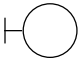
\includegraphics[width=0.09\textwidth]{BoundaryClass}
\end{wrapfigure}
Separate the interfaces from the rest of the system. Handles communication with the environment (users and other systems)
\subsubsection{Entity Class}
\begin{wrapfigure}[3]{r}{0.1\textwidth}
    
\includegraphics[width=0.09\textwidth]{EntityClass}
\end{wrapfigure}
Functionality dealing with the storage and handling of long-lived (potential persistent) information. Often are general to many use cases
\subsubsection{Control Class}
\begin{wrapfigure}[3]{r}{0.1\textwidth}
    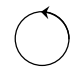
\includegraphics[width=0.09\textwidth]{ControlClass}
\end{wrapfigure}
Controls interactions between a group of objects. Functionality specific to one, or a few use cases, and not naturally placed in the other class types
\subsection{Relationships between Classes}
\subsubsection{Association}
Defines a semantic relationship between classes. An association has; a name, at least two association end, each end attached to a class.\\
\textbf{Aggregation} -- variation of the ``has a'' association relationship\\
\textbf{Composition} -- can exist via a part of (e.g. Carburettor ``is a part of'' Car)\\
\textbf{Generalisation} -- defines inheritance between a super and sub class

\section{State Machine}
\textbf{Moore} -- actions associated with states or transitions\\
\textbf{Mealy} -- actions may depend on system state as well as trigger\\
\textbf{Quantitative} state is the current values of all of an object's attributes\\
\textbf{Qualitative} state is the current status of an object during its lifespan\\
\subsection{Notation}
\subsubsection{State}
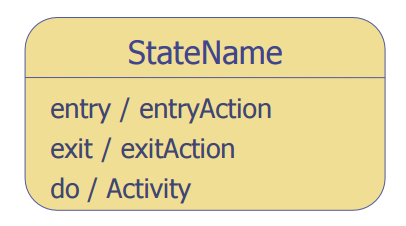
\includegraphics[width=0.3\textwidth]{State}
\subsubsection{State Transition}
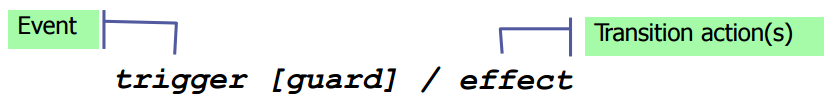
\includegraphics[width=0.3\textwidth]{Transition}

\section{Measurement}
\subsection{What can we measure}
\subsubsection{Products}
System (size, defect, density), Module (length, percent reused, independent flow paths), Defect (type, origin, detection, severity, effort to fix)
\subsubsection{Processes}
Development (elapsed time, effort, phase containment), Testing (tests passed), Maintenance (staff hours per request)
\subsubsection{Projects}
Resources, Progress relative to schedule, Productivity, Product characteristics, Process characteristics
\subsection{Structure-Related Metrics}
Problem Complexity, Algorithm Complexity (time and space), Structural Complexity (control flow, data flow), Cognitive Complexity (human understanding)
\subsection{Measurement Etiquette}
\subsubsection{Do}
\begin{itemize}
    \item Use common sense and organisational sensitivity when interpreting metrics data
    \item Provide regular feedback to the individuals and teams who have collected the data
    \item Work with engineers and teams to set clear goals and the metrics that will be used to measure them
\end{itemize}
\subsubsection{Don't}
\begin{itemize}
    \item Don't use metrics to appraise individuals
    \item Never use metrics to threaten teams or individuals
    \item Don't obsess about a single metric to the exclusion of others
    \item Don't treat metrics data that identifies a problem as ``negative''
\end{itemize}

\section{Software Estimation}
\subsection{How to Estimate}
\subsubsection{Analogy}
Identify similar projects and estimate based on these previous projects. Accuracy can be improved by partitions the project and estimating each part. \textit{International Software Benchmarking Standards Group (ISBSG)}
\subsubsection{Wide-band Delphi}
Get multiple experts/stakeholders, each person give estimation anonymously.
\subsection{Software Size Measures}
Syntactic (e.g. Lines of Code (LOC, KLOC)), Semantic (e.g. Function Points)
\subsubsection{Function Points}
Developed by Albrecht (1979). Based on a user view of the system:
\begin{itemize}
    \item \textbf{External Inputs} -- input screen
    \item \textbf{External Outputs} -- output screen
    \item \textbf{External Enquiries} -- prompt for input
    \item \textbf{Internal Logical Files} -- database table
    \item \textbf{External Interface Files} -- database table shared between applications
\end{itemize}
\begin{equation*}
    \text{Function Points} = 4\times EI+5\times EO+4\times EQ+10\times ILF+7\times EIF
\end{equation*}
\subsection{Simple Estimation Technique}
Each entity class in a model will need; 1 user interface, 1 data access, half helper class. Assumes you know developer productivity (typical: 2 - 20 classes/month, average: 4 - 8)
\begin{equation*}
    E=3.5\times\frac{\text{Model Classes}}{\text{Productivity}}
\end{equation*}
\subsection{COCOMO 2}
Developed by Barry Boehm
\subsubsection{Application Points}
Number of separate screens displayed (simple=1, average=2, complex=3). Number of reports produced (simple=2, average=5, complex=8). Number of 3GL modules that must be developed to supplement the 4GL code (10 object points per module)
\subsubsection{Formula}
\begin{equation*}
    PM= \frac{NAP\times\left(1 - \frac{\%reuse}{100}\right)}{PROD}
\end{equation*}
PM -- effort in person-months. NAP -- number of application points. PROD -- productivity
(Developer Experience and Capability / CASE Maturity and Capability, PROD), (V Low, 4), (Low, 7), (Nominal, 13), (High, 25), (V High, 50)
\subsubsection{Multipliers}
\begin{wrapfigure}[8]{r}{0.2\textwidth}
    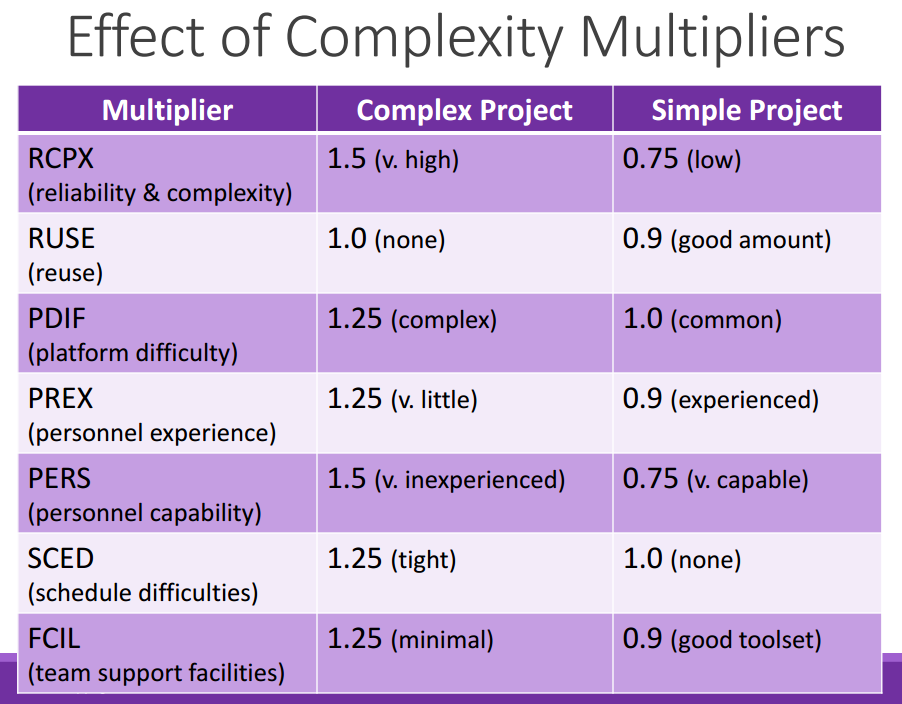
\includegraphics[width=0.19\textwidth]{Effect}
\end{wrapfigure}
RCPX -- product reliability and complexity. RUSE -- reuse required. PDIF -- platform difficulty. PREX -- personnel experience. PERS -- personnel capability. SCED -- required schedule. FCIL -- team support facilities


\vfill\vspace{1em}\textit{Written by Daniel Fitz}
\end{multicols}
\end{landscape}
\end{document}
